\documentclass{article}

\usepackage{float,algorithm,graphicx,amsmath,amsfonts,verbatim,hyperref}
\usepackage[noend]{algpseudocode}

\title{Lab 11 - Reinforcement Learning}
\author{Kyle Swanson}
\date{January 30, 2018}

\setcounter{section}{-1}

\begin{document}

\maketitle

\section{Introduction}

\subsection{Overview}

Today's lab will be exploring reinforcement learning, which involves methods for learning how to perform a task or play a game. The goal is to learn a policy $\pi(s)$ which outputs an action $a$ for each state $s$. For instance, in a game of Pong, the state would be the location of the two paddles and the location of the ball, and the action would be whether to move the paddle up or down. To determine how well a policy performs, we measure how much reward is gained by following the actions specified by the policy. For Pong, the reward would be how many goals we score. We are going to use reinforcement learning techniques to learn the optimal policy $\pi^*(s)$ which outputs the action $a$ which will lead to the greatest reward for each state $s$ (e.g. for Pong we try to learn whether moving the paddle up or down will lead us to score the most goals, given the current positions of the paddle and the ball).

\subsection{CartPole}

In this lab, we are going to be learning how to play a simple game called CartPole (see image below).

\noindent
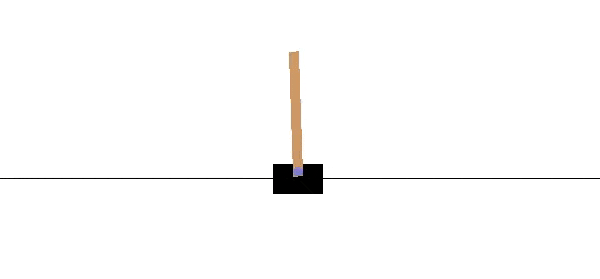
\includegraphics[width=\textwidth]{cartpole.png}

In CartPole, we have a cart (black box) which is trying to balance a pole (brown line). The only actions we can take are we can move the box to the left or to the right. Our reward is how long we're able to keep the pole balanced before it falls over. The state of the game consists of four features:

\begin{enumerate}
    \item Cart position
    \item Cart velocity
    \item Pole angle
    \item Pole velocity at tip
\end{enumerate}

\noindent
At each step in the game, we are given these four features as the current state, and we need to make a decision about what action to take (moving the cart left or right). The full CartPole game specification is here: \url{https://github.com/openai/gym/wiki/CartPole-v0}

In this lab, we are going to try three methods for playing this game. First we'll build a random agent which will randomly move the cart to the left or to the right on each step. We'll see that this policy performs very poorly. Then we'll build a hand-engineered agent, where you will manually design an algorithm to select an action based on the state. It is possible to play the game well using a hand-engineered agent, but it takes some work. Finally, we will use a type of reinforcement learning called Deep Q-Networks (DQN), which use neural networks to learn how to predict the best action by playing the game many times over and learning to predict actions lead to the greatest reward. At first the DQN agent performs poorly, but as it trains, its performance improves, and after 10-15 minutes it can play like an expert.

\subsection{Installation}

Install gym, which generates game environments that we can learn to play:

\vspace{2mm}

\noindent
\texttt{pip install gym}

\vspace{2mm}

In order to save short GIFs of your agent playing the game, install ImageMagick: \url{https://www.imagemagick.org/script/download.php}

If you're having trouble installing ImageMagick, set \texttt{gif\_path=None} each of the times it appears in \texttt{main.py} so that your code won't crash when it tries to save GIFs without ImageMagick installed. You will still be able to see your agent play the game, but the GIF will not be saved.

\section{Reinforcement Learning}

\subsection{Random Agent}

First we are going to build an agent which will take random actions on each step, meaning it will randomly decide whether to move the cart to the left or to the right.

Go into \texttt{lab11.py} and find the \texttt{RandomAgent} class. Your job is to implement the \texttt{act} method, which takes in a state and outputs an action. The state is going to be a gym observation object, and the action should be an integer in the range from \texttt{0} to \texttt{self.action\_size - 1}. In the case of CartPole, \texttt{self.action\_size = 2}, so the possible actions are \texttt{0} (push the cart to the left) and \texttt{1} (push the cart to the right). For the \texttt{RandomAgent} act method, you should ignore the provided state and just randomly return either \texttt{0} or \texttt{1}. This will randomly push the cart either to the left or to the right on each step.

Once your implementation is complete, go into \texttt{main.py}, uncomment Part 1.1, and run the code. You should see a quick animation of CartPole, which lasts for maybe half a second. This is your \texttt{RandomAgent} controlling the cart, but almost right away the pole tips too far and the game ends.

If you were able to install ImageMagick, a GIF of the game will be saved as \texttt{random.gif}. You can open this GIF to watch the \texttt{RandomAgent} playing the game on loop. If you weren't able to install ImageMagick, change \texttt{gif\_path='random.gif'} to \texttt{gif\_path=None} so that your code doesn't crash. You'll still be able to see the animation, but the GIF won't be saved.

\subsection{Engineered Agent}

Randomly pushing the cart left or right is obviously a bad policy, so let's try to come up with something better. We're not going to use machine learning yet; instead, this section is an opportunity for you to try to hand-engineer an agent to play CartPole.

Go into \texttt{lab11.py} and find the \texttt{EngineeredAgent} class. As with the \texttt{RandomAgent}, your goal is to take in the current state and return an action (\texttt{0} or \texttt{1}). I've extracted the different components of the state for you. Manually design an algorithm to use the state to decide what action to make.

When testing your algorithm, go into \texttt{main.py}, uncomment Part 1.2, and run the code. See how long your algorithm is able to balance the pole. It takes some work, but it is possible to manually design the \texttt{act} method to play the game almost perfectly. If you aren't able to get a perfect agent, don't worry about it. This section is intended to give you a sense of the challenges inherent in CartPole, so you'll have a better sense of what our reinforcement learning algorithm needs to learn.

\subsection{Deep Q-Network (DQN) Agent}

Now we will use a reinforcement learning algorithm called Deep Q-Networks (DQN) to learn how to play CartPole. While the DQN agent takes less than 100 lines of code to implement (ignoring comments), it's a little tricky to get it right so I've provided an implementation for you, based on the implementation here: \texttt{https://github.com/keon/deep-q-learning/blob/master/dqn.py} For a good explanation of how the code works, check out this tutorial: \texttt{https://keon.io/deep-q-learning/}

Go into \texttt{main.py}, uncomment Part 1.3, and run the code. You'll see that the neural network in the DQN agent will start to train by playing episodes of the game and learning which actions lead to the most reward. The DQN will be trained for 2000 episodes, and an animation of its current policy will be displayed after every 100 episodes. You'll see that at first the agent performs very poorly, much like the random agent, but over time it begins to discover methods for balancing the pole. By the end of 2000 episodes, it should be able to play CartPole very well. That's the power of reinforcement learning.

(Note: Since the training procedure involves some randomness, the DQN agent doesn't always learn the same techniques and may, on occasion, learn a bad policy. If your agent isn't performing well after 2000 episodes, you can try running the code again, and hopefully you'll get luckier the next time.)

\end{document}
